%%% Template originaly created by Karol Kozioł (mail@karol-koziol.net) and modified for ShareLaTeX use

\documentclass[a4paper,11pt]{article}

\usepackage[T1]{fontenc}
\usepackage[utf8]{inputenc}

\usepackage{xcolor}
\usepackage{parskip}
\usepackage{tgtermes}
\usepackage{graphicx,wrapfig,lipsum}
\usepackage[
pdftitle={Math Assignment}, 
pdfauthor={Lucas Varela, Universidad de los Andes},
colorlinks=true,linkcolor=blue,urlcolor=blue,citecolor=blue,bookmarks=true,
bookmarksopenlevel=2]{hyperref}
\usepackage{amsmath,amssymb,amsthm,textcomp}
\usepackage{enumerate}
\usepackage{multicol}
\usepackage{tikz}

\usepackage{geometry}
\geometry{total={210mm,297mm},
left=25mm,right=25mm,%
bindingoffset=0mm, top=20mm,bottom=20mm}

\linespread{0.9}

\newcommand{\linia}{\rule{\linewidth}{0.5pt}}

% custom theorems if needed
\newtheoremstyle{mytheor}
    {1ex}{1ex}{\normalfont}{0pt}{\scshape}{.}{1ex}
    {{\thmname{#1 }}{\thmnumber{#2}}{\thmnote{ (#3)}}}

\theoremstyle{mytheor}
\newtheorem{defi}{Definition}

% my own titles
\makeatletter
\renewcommand{\maketitle}{
\begin{center}
\vspace{2ex}
{\huge \textsc{\@title}}
\vspace{1ex}
\\
\linia\\
\@author \hfill \@date
\vspace{4ex}
\end{center}
}
\makeatother
%%%

% custom footers and headers
\usepackage{fancyhdr,lastpage}
\pagestyle{fancy}
\lhead{}
\chead{}
\rhead{}
\lfoot{Solución problema Kleppner 4.23}
\cfoot{}
\rfoot{Page \thepage\ /\ \pageref*{LastPage}}
\renewcommand{\headrulewidth}{0pt}
\renewcommand{\footrulewidth}{0pt}
%

%%%----------%%%----------%%%----------%%%----------%%%

\begin{document}

\title{Complementaria de Física I -- Taller Semana 11}

\author{Universidad de los Andes}

\date{}

\maketitle

\color{blue}

\begin{figure}[h]
	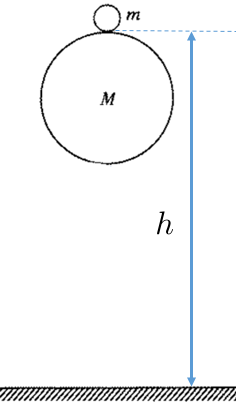
\includegraphics[width=.2\linewidth]{1}
	\label{fcN4}
\end{figure}

\color{blue}
\paragraph{Kleppner 4.23} Una bola de masa $M$ y otra de masa $m$ se sueltan juntas desde una altura $h$ del suelo ($h$ se mide desde el suelo hasta el punto de contacto entre las bolas). Encuentre la altura máxima que alcanza la bola pequeña sabiendo que $m$ es mucho menos masiva que $M$ ($m\ll M$). Suponga que todas las colisiones son elásticas.


\color{black}

\textbf{Solución}

Primero calculemos con cuanta velocidad llega la pelota al suelo. Al ser caída libre se encuentra por conservación de energía que la velocidad con la que llega es:

$$v^2 = 2gh$$

Esta también es la velocidad con la que llega la pelota pequeña (recuerde que en caída libre la velocidad final no depende de la masa). Ahora como la colisión con el piso es elástica, la energía antes y después de la colisión es la misma, por lo que la pelota $M$ rebota y sale con la misma rapidez pero con la dirección opuesta. Entonces vemos que después de que la pelota $M$ rebota se tiene la siguiente situación mostrada en el dibujo.

\begin{figure}[h]
	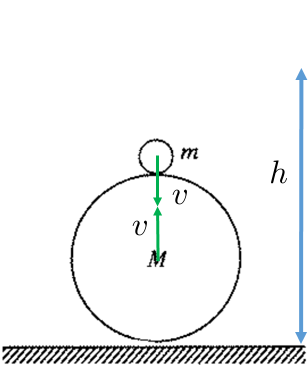
\includegraphics[width=.3\linewidth]{2}
	\label{fcN4}
\end{figure}

Entonces ambas pelotas se mueven con la misma rapidez pero la dirección contraria. Por lo tanto justo antes de la colisión entre las bolas se tiene el siguiente momento lineal en la dirección $y$:

$$ p_{y_i} = M v - m v = (M-m)v$$

y la energía es:

$$ E_i= \frac{1}{2} M v^2 + \frac{1}{2} m v^2 = \frac{1}{2} (M+m) v^2 $$

Ahora miremos justo después de la colisión que pasa.

\begin{figure}[h]
	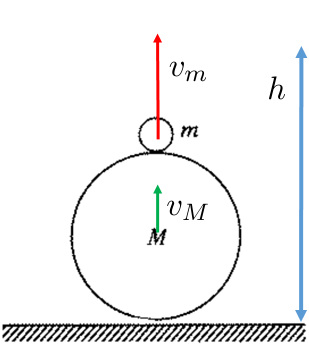
\includegraphics[width=.3\linewidth]{3}
	\label{fcN4}
\end{figure}

Después de la colisión se tiene el siguiente momento lineal en $y$:


$$ p_{y_f} = M v_M + m v_m $$

Y la siguiente energía
$$ E_f= \frac{1}{2} M v_M^2 + \frac{1}{2} m v_m^2 $$

Como se esta mirando el momento justo antes y justo después de la colisión, la gravedad no tiene tiempo para cambiar el momento lineal en $y$ y se tiene que $p_{y_f} = p_{y_i} $. De esto sigue que:

$$ (M-m)v = M v_M + m v_m $$


Nos interesa saber $v_m$ por lo que despejamos $v_M$ en términos de dicha cantidad:


$$  v_M =  \left(1-\frac{m}{M}\right)v -  \frac{m}{M} v_m $$


Ahora como suponemos este choque también fue elástico, se conserva la energía, es decir $E_f = E_i$ por lo que se tiene:

$$ \frac{1}{2} (M+m) v^2 = \frac{1}{2} M v_M^2 + \frac{1}{2} m v_m^2 $$

O multiplicando por 2:

$$  (M+m) v^2 =  M v_M^2 +  m v_m^2 $$


Ahora calculamos $v_M^2$ con la expresión que obtuvimos de conservación de momento.


\begin{align*}
v_M^2 & = \left( \left(1-\frac{m}{M}\right)v -  \frac{m}{M} v_m \right)^2 \\
& =    \left(1-\frac{m}{M}\right)^2v^2 -2\frac{m}{M} \left(1-\frac{m}{M}\right) v v_m + \frac{m^2}{M^2} v_m^2\\
& = v^2 - 2\frac{m}{M} v^2 + \frac{m^2}{M^2}v^2 - 2\frac{m}{M} v v_m + 2\frac{m^2}{M^2} v v_m  + \frac{m^2}{M^2} v_m^2
\end{align*}

Ahora usamos la suposición que $M$ es mucho más grande que $m$. Si esto pasa entonces $m/M$ es muy pequeño y $m^2/M^2$ aun más pequeño. Por lo tanto vamos a hacer la aproximación $m^2/M^2 \approx 0$. Por lo tanto se tiene que:


$$ v_M^2 \approx v^2 -  2\frac{m}{M} v^2 - 2\frac{m}{M} v v_m $$

Reemplazando esto en la ecuación de conservación de energía:

$$  (M+m) v^2 =  M  \left(v^2 -  2\frac{m}{M} v^2 - 2\frac{m}{M} v v_m\right) +  m v_m^2 $$

Simplificando:

$$  (M+m) v^2 =  M  v^2 -  2m v^2 - 2m v v_m +  m v_m^2 $$

Y simplificando aún más:

$$ v_m^2 - 2 v v_m  - 3v^2 = 0$$

Las soluciones para ésta cuadrática son:

$$ v_m = {v \pm 2 v} $$

Pero no tiene sentido que la pelota salga con velocidad negativa por lo que se tiene una velocidad final para $m$ dada por:

$$ v_m = 3v$$

Ahora usando conservación de energía, se tiene que la energía cuando la pelota llegue a su altura máxima sera solo potencial $E = mg H$. Su energía justo después del choque es solo cinética $E = 1/2 m v_m^2$. Por lo tanto:

$$ H = \frac{v^2_m}{2g} = \frac{9 v^2}{2g} = 9h$$

\begin{figure}[h]
	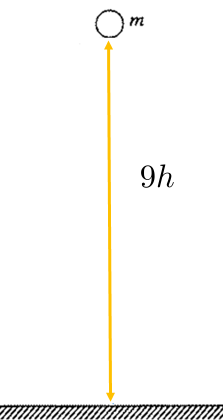
\includegraphics[width=.23\linewidth]{4}
	\label{fcN4}
\end{figure}

\end{document}
